% Common
\documentclass[12pt,a4paper,oneside]{article}
\usepackage[left=2cm, right=2cm, top=2.5cm, bottom=2.5cm]{geometry}
\usepackage[ngerman]{babel}
\usepackage[utf8]{inputenc}

% Header
\usepackage{fancyhdr}

% Math
\usepackage{amsmath}
\usepackage{amsfonts}
\usepackage{amssymb}
\usepackage{paralist}

% include PDF-Pages
\usepackage[final]{pdfpages}

\usepackage{subfigure}
\usepackage{graphicx}
\usepackage{listings}
\usepackage{color}
\usepackage{xcolor}

% Table rules
%\usepackage{booktabs}

\title{Weihnachtsübung\\
  \textbf{Numerik
  }
}

\author{Thorsten Weber\\
  Matr.-Nr.: 344219\\
  \\Max Stachon\\
  Matr.-Nr.: 344173\\
  \\Gerrit Toehgiono\\
  Matr.-Nr.: 343666
}

\date{\today}

% HEADER / FOOTER
\pagestyle{fancy}
\fancyhf{}
\rhead{Seite \thepage}
\lhead{Numerik -- Weihnachtsübung}
\cfoot{\footnotesize Thorsten Weber (344219), Max Stachon (344173), Gerrit Toehgiono (343666)}

\renewcommand{\headrulewidth}{1pt}
\renewcommand{\footrulewidth}{1pt}

\begin{document}
\clearpage
\maketitle
\thispagestyle{empty}
\newpage

\section*{Aufgabe 1}
Benutzter Code: \\
\begin{lstlisting}[language=Matlab,frame=single]
function [ DUI , DDI ] = kantendetektion(I)

%Umwandeln der Matrix I in double
I = double(I);
%I = I / 255;
%Festlegen von m und n (Dimension der Matrix)
D = size(I);
n = D(1,1);
m = D(1,2);

%Fuellen der neuen Matrix mit nullen
DDI = zeros(n,m);
DUI = zeros(n,m);

% 2.1 Randbedingungen Erweitere die Matrix wie in 2.1 beschrieben
I1 = I(1,:);
I = [I1;I];
I2 = I(end,:);
I = [I;I2];
I3 = I(:,1);
I = [I3,I];
I4 = I(:,n);
I = [I,I4];

%Aufstellen des Gradienten
for i = 2:n+1;
for j = 2:m+1;
    T1 = (1/2*(I(i+1,j)-I(i,j) + I(i+1,j+1) - I(i,j+1)));
    T2 = (1/2*(I(i,j+1)-I(i,j) + I(i+1,j+1) - I(i+1,j)));
    %Multiplikation von Gradient^T * Gradient
    DDI(i-1,j-1) = [T1,T2] * [T1;T2];    
end
end

%Differenzenquotient berechnen
for i = 2:n+1;
for j = 2:m+1;
    %Formel aus Tabelle 2
    DUI(i-1,j-1) = I(i,j+1)+I(i,j-1)+I(i+1,j)+I(i-1,j)-4*I(i,j);
end
end
\end{lstlisting}
\textbf{Eingabe in Funktion:} [DUI, DDI] = kantendetektion(imread('bilder/drei.bmp'))


\begin{figure} 
\textbf{Ausgabe:} imshow(DDI) und imshow(DUI)\\
    \subfigure[Gradient]{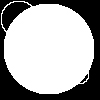
\includegraphics[width=0.49\textwidth]{bilder/Aufgabe1/Kantendetektion/gradient_drei.jpg}} 
    \subfigure[Differenzenquotient]{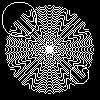
\includegraphics[width=0.49\textwidth]{bilder/Aufgabe1/Kantendetektion/laplace_drei.jpg}} 
\caption{Kantendetektion drei.bmp} 

 \subfigure[Gradient]{
\includegraphics[width=0.49\textwidth]{bilder/Aufgabe1/Kantendetektion/gradient_rau.jpg}} 
    \subfigure[Differenzenquotient]{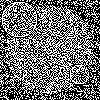
\includegraphics[width=0.49\textwidth]{bilder/Aufgabe1/Kantendetektion/laplace_rau.jpg}} 
\caption{Kantendetektion rau.bmp} 
\end{figure} 

\newpage






\begin{figure} 
\section*{Aufgabe 2}
Code zur Schwellenwertbinarisierung:
\begin{lstlisting}[language=Matlab,frame=single]

%Enter x, y as SCHWELLENWERT and I as Matrix to detect.
%Fuer zwei Kreise nutze imshow(schwellenwert(15,50,DUI))
%Fuer grossen Kreis nutze imshow(schwellenwert(-18,-2,DUI))

function [ T ] = schwellenwert( x, y, I )

D = size(I);
n = D(1,1);
m = D(1,2);



for i = 1:n;
for j = 1:m;
    if I(i,j) > x && I(i,j) < y
        T(i,j) = 0;
    else
        T(i,j) = 1;
    end
end
end

end

\end{lstlisting}

\textbf{Ausgabe:\\}
    \subfigure[imshow(schwellenwert(15,50,DUI)]{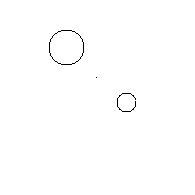
\includegraphics[width=0.49\textwidth]{bilder/Aufgabe2/klein.jpg}} 
    \subfigure[imshow(schwellenwert(-18,-2,DUI)]{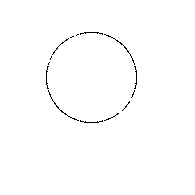
\includegraphics[width=0.49\textwidth]{bilder/Aufgabe2/gross.jpg}} 
\caption{Schwellenwertbinarisierung} 
\end{figure} 

\newpage

\begin{figure} 
\section*{Aufgabe 3}
Code zum Entrauschen:
\begin{lstlisting}[language=Matlab,frame=single]
function [ I ,DUI ] = entrauschen()
%Einlesen des Bildes
 I = double(imread('bilder\rau.bmp', 'BMP'));
 I = I / 255;
D = size(I);
n = D(1,1);
m = D(1,2);

for z = 1:250
    %Entrauschen des Bildes ueber die bereits vorhandenen Funktionen
[DUI, DDI] = kantendetektion( I);
DUI = double(DUI);
   
   DUI = 0.006 * DUI;
   I = I + DUI;
end
%ACHTUNG kann zu Skalierungsproblemen kommen.
%Je nach Einstellung von imshow!
%ggf Werte der Matrix durch Multiplikation erhoehen.


\end{lstlisting}

\textbf{Ausgabe:\\}
    \subfigure[Gradient]{
\includegraphics[width=0.49\textwidth]{bilder/Aufgabe3/gradient_rau.jpg}} 
    \subfigure[Differenzenquotient]{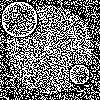
\includegraphics[width=0.49\textwidth]{bilder/Aufgabe3/laplace_rau.jpg}} 
\caption{Schwellenwertbinarisierung} 
\end{figure} 

\newpage

\begin{figure} 
\section*{Aufgabe 4}
Code zum Binarisieren des Bildes:
\begin{lstlisting}[language=Matlab,frame=single]
function [ T] = kantendetektionBild(x,y)
%imshow(kantendetektionBild(-70,40))
 [I ,DI ] = kantendetektion(imread('bilder\camera.bmp'));
 
 D = size(I);
n = D(1,1);
m = D(1,2);

for i = 1:n;
for j = 1:m;
    if I(i,j) > x && I(i,j) < y
        T(i,j) = 1;
    else
        T(i,j) = 0;
    end
end
end
end


\end{lstlisting}

\textbf{Ausgabe je nach Schwellenwert:\\}
    \subfigure[Ausgabe 1]{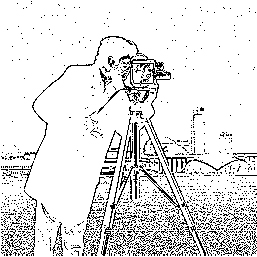
\includegraphics[width=0.49\textwidth]{bilder/Aufgabe4/MannMitStativ.jpg}} 
    \subfigure[Ausgabe 2]{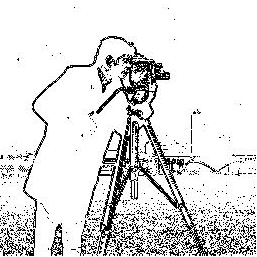
\includegraphics[width=0.49\textwidth]{bilder/Aufgabe4/mann.jpg}} 
\caption{Schwellenwertbinarisierung eines Bildes} 

\end{figure} 

\newpage

\begin{figure} 
\section*{Aufgabe 5}
Code zum Optischen Fluss:
\begin{lstlisting}[language=Matlab,
frame=single,breaklines=true,keepspaces=true]



function [ I ] = bewegung()
%Einlesen der Bilder
I1 = double(imread('bilder\bewegung1.bmp', 'BMP'));
I2 = double(imread('bilder\bewegung2.bmp', 'BMP'));

%Berechnung der Dimension
D = size(I1);
n = D(1,1);
m = D(1,2);

% 2.1 Randbedingungen Erweitere die Matrix 1.

I11 = I1(1,:);
I1 = [I11;I1];
I21 = I1(end,:);
I1 = [I1;I21];
I31 = I1(:,1);
I1 = [I31,I1];
I41 = I1(:,end);
I1 = [I1,I41];
% 2.1 Randbedingungen Erweitere die Matrix 2.
I12 = I2(1,:);
I2 = [I12;I2];
I22 = I2(end,:);
I2 = [I2;I22];
I32 = I2(:,1);
I2 = [I32,I2];
I42 = I2(:,end);
I2 = [I2,I42];

%Berechnung von Ix Iy und It
for i = 2:n+1;
for j = 2:m+1;
    Ix(i-1,j-1) = (1/4 * (I1(i+1,j)-I1(i,j)+I1(i+1,j+1)-I1(i,j+1)+I2(i+1,j)-I2(i,j)+I2(i+1,j+1)-I2(i,j+1)));
    Iy(i-1,j-1) = (1/4 * (I1(i,j+1)-I1(i,j)+I1(i+1,j+1)-I1(i+1,j)+I2(i,j+1)-I2(i,j)+I2(i+1,j+1)-I2(i+1,j)));
    It(i-1,j-1) = (1/4 * (I2(i,j+1)-I1(i,j+1)+I2(i+1,j+1)-I1(i+1,j+1)+I2(i+1,j)-I1(i+1,j)+I2(i,j)-I1(i,j)));
        
end
end


\end{lstlisting}


\end{figure} 

\newpage

\begin{figure} 

Code zum Optischen Fluss Fortsetzung:
\begin{lstlisting}[language=Matlab,
frame=single,breaklines=true,keepspaces=true]

%Erweitere Matrix um 2 Stellen je Seite;
Ix = [ones(2,100);Ix;ones(2,100)];
Ix = [ones(104,2),Ix,ones(104,2)];

Iy = [ones(2,100);Iy;ones(2,100)];
Iy = [ones(104,2),Iy,ones(104,2)];

It = [ones(2,100);It;ones(2,100)];
It = [ones(104,2),It,ones(104,2)];


%Erstelle nun Ausgleichsproblem mit Loesung.
for i = 3:n+2;
for j = 3:m+2;
    
   a1 = Ix(i-2,j-2); b1 = Ix(i-2,j-1); c1 = Ix(i-2,j); d1 = Ix(i-2,j+1); e1 = Ix(i-2,j+2);
   a2 = Ix(i-1,j-2); b2 = Ix(i-1,j-1); c2 = Ix(i-1,j); d2 = Ix(i-1,j+1); e2 = Ix(i-1,j+2);
   a3 = Ix(i,j-2);   b3 = Ix(i,j-1);   c3 = Ix(i,j);   d3 = Ix(i,j+1);   e3 = Ix(i,j+2);
   a4 = Ix(i+1,j-2); b4 = Ix(i+1,j-1); c4 = Ix(i+1,j); d4 = Ix(i+1,j+1); e4 = Ix(i+1,j+2);
   a5 = Ix(i+2,j-2); b5 = Ix(i+2,j-1); c5 = Ix(i+2,j); d5 = Ix(i+2,j+1); e5 = Ix(i+2,j+2);
    
  Px = [a1 b1 c1 d1 e1 a2 b2 c2 d2 e2 a3 b3 c3 d3 e3 a4 b4 c4 d4 e4 a5 b5 c5 d5 e5];
  
   a1 = Iy(i-2,j-2); b1 = Iy(i-2,j-1); c1 = Iy(i-2,j); d1 = Iy(i-2,j+1); e1 = Iy(i-2,j+2);
   a2 = Iy(i-1,j-2); b2 = Iy(i-1,j-1); c2 = Iy(i-1,j); d2 = Iy(i-1,j+1); e2 = Iy(i-1,j+2);
   a3 = Iy(i,j-2);   b3 = Iy(i,j-1);   c3 = Iy(i,j);   d3 = Iy(i,j+1);   e3 = Iy(i,j+2);
   a4 = Iy(i+1,j-2); b4 = Iy(i+1,j-1); c4 = Iy(i+1,j); d4 = Iy(i+1,j+1); e4 = Iy(i+1,j+2);
   a5 = Iy(i+2,j-2); b5 = Iy(i+2,j-1); c5 = Iy(i+2,j); d5 = Iy(i+2,j+1); e5 = Iy(i+2,j+2);
   
   Py = [a1 b1 c1 d1 e1 a2 b2 c2 d2 e2 a3 b3 c3 d3 e3 a4 b4 c4 d4 e4 a5 b5 c5 d5 e5];
   
   A = [Px' , Py'];
 
\end{lstlisting}




\end{figure} 

\newpage

\begin{figure} 

Code zum Optischen Fluss Fortsetzung:
\begin{lstlisting}[language=Matlab,
frame=single,breaklines=true,keepspaces=true]
   
   a1 = It(i-2,j-2); b1 = It(i-2,j-1); c1 = It(i-2,j); d1 = It(i-2,j+1); e1 = It(i-2,j+2);
   a2 = It(i-1,j-2); b2 = It(i-1,j-1); c2 = It(i-1,j); d2 = It(i-1,j+1); e2 = It(i-1,j+2);
   a3 = It(i,j-2);   b3 = It(i,j-1);   c3 = It(i,j);   d3 = It(i,j+1);   e3 = It(i,j+2);
   a4 = It(i+1,j-2); b4 = It(i+1,j-1); c4 = It(i+1,j); d4 = It(i+1,j+1); e4 = It(i+1,j+2);
   a5 = It(i+2,j-2); b5 = It(i+2,j-1); c5 = It(i+2,j); d5 = It(i+2,j+1); e5 = It(i+2,j+2);
   
   b = -1 * [a1 b1 c1 d1 e1 a2 b2 c2 d2 e2 a3 b3 c3 d3 e3 a4 b4 c4 d4 e4 a5 b5 c5 d5 e5]';  
   %Berechne x Stern
   M = pinv(A);
   %xs ist der Vektor mit u und v
   xs =  M * b;
    u(i-2,j-2) = xs(1,1);
    v(i-2,j-2) = xs(2,1);
   
   I(i-2,j-2) = norm(((A * xs) - b),2);
         
end
end


quiver(v(1:10:end,1:10:end),u(1:10:end,1:10:end))
end

\end{lstlisting}

\textbf{Ausgabe des Optischen Flusses:\\}
    \subfigure[Ausgabe 1]{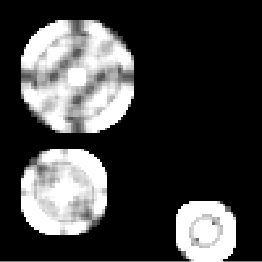
\includegraphics[width=0.49\textwidth]{bilder/Aufgabe5/bewegungImg.jpg}} 
    \subfigure[Ausgabe 2]{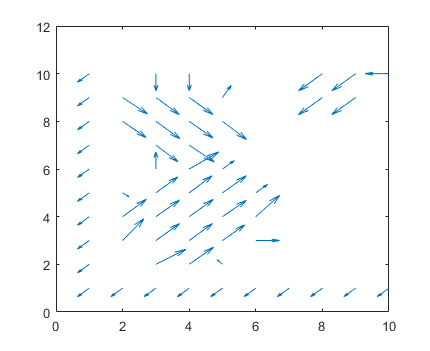
\includegraphics[width=0.49\textwidth]{bilder/Aufgabe5/optischerFluss.jpg}} 



\end{figure} 

\end{document}
